

\documentclass[12pt,a4paper,oneside,pdftex]{report}


\usepackage{subcaption}
\usepackage{graphicx}
\usepackage{amsmath}

\usepackage{tikz}
\usetikzlibrary{positioning}
\usetikzlibrary{calc}
\usetikzlibrary{arrows}
\usetikzlibrary{decorations.pathmorphing,decorations.markings}
\usetikzlibrary{shapes}
\usetikzlibrary{patterns}
\usetikzlibrary{automata}

\tikzset{
c/.style={
  circle,
  inner sep=0pt,
  text width=6mm,
  align=center,
  draw=black,
  fill=white
  }
}


\begin{document}

\begin{figure}
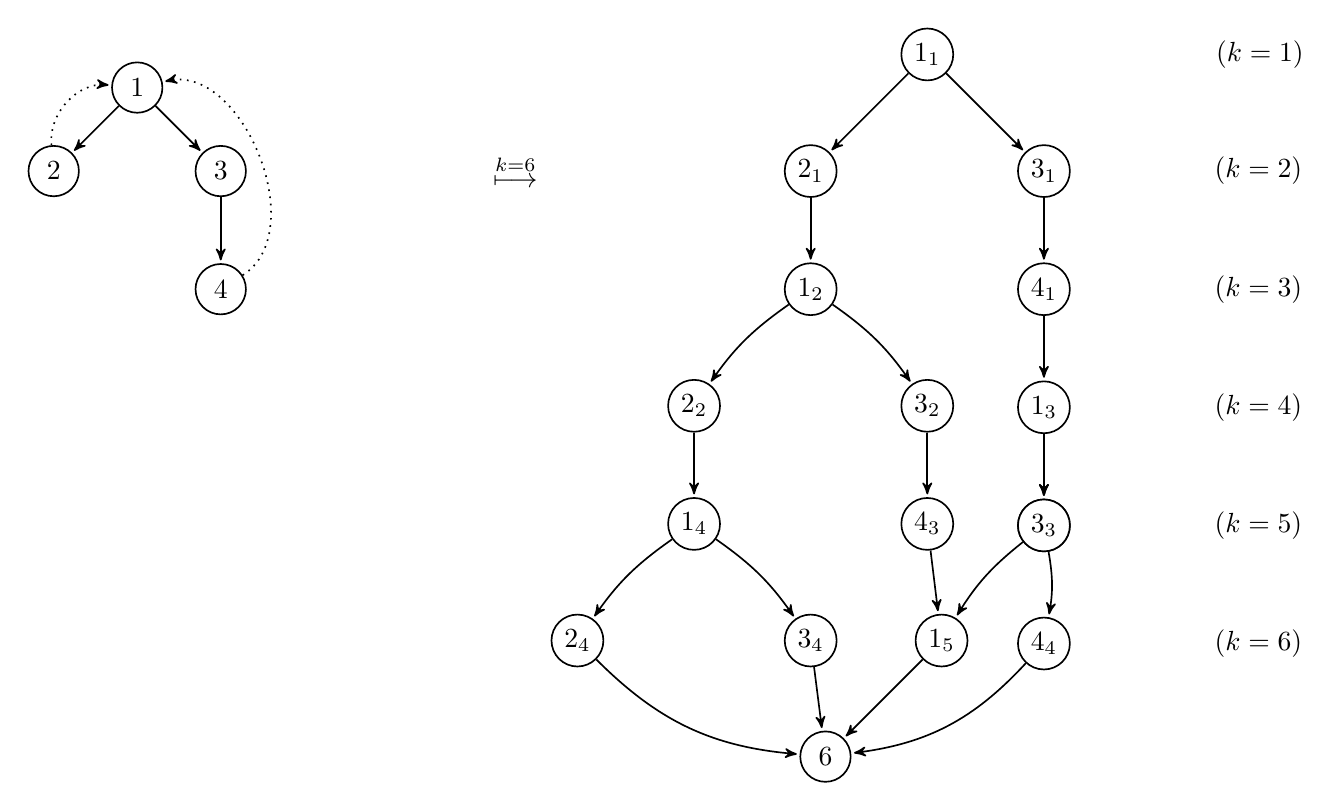
\begin{tikzpicture}[->,>=stealth',shorten >=1pt,auto,node distance=1.5cm,semithick]
\node[c] (1) [] {$1$};
\node[c] (2) [below left of=1] {$2$};
\node[c] (3) [below right of=1] {$3$};
\node[c] (4) [below of=3] {$4$};
\path[->]
(1) edge [] node {} (2)
(2) edge [bend left=50,dotted] node {} (1)
(1) edge [] node {} (3)
(3) edge [] node {} (4)
(4) edge [bend right=80,dotted] node {} (1)
;
\node[draw=none] (impl) [right=3cm of 3] {$\overset{k = 6}{\longmapsto}$};
;
\node[c] (21) [right=3cm of impl] {$2_1$};
\node[c] (11) [above right=1cm and 1cm of 21]{$1_1$};
\node[c] (31) [below right=1cm and 1cm of 11] {$3_1$};
\node[c] (41) [below of=31] {$4_1$};
\node[c] (12) [below of=21] {$1_2$};
\node[c] (22) [below left=1cm and 1cm of 12] {$2_2$};
\node[c] (32) [below right=1cm and 1cm of 12] {$3_2$};
\node[c] (13) [below of=41] {$1_3$};
\node[c] (14) [below of=22] {$1_4$};
\node[c] (43) [below of=32] {$4_3$};
\node[c] (23) [below of=13] {$2_3$};
\node[c] (33) [below of=13] {$3_3$};
\node[c] (24) [below left=1cm and 1cm of 14] {$2_4$};
\node[c] (34) [below right=1cm and 1cm of 14] {$3_4$};
\node[c] (15) [below right=1cm and -0.3cm of 43] {$1_5$};
\node[c] (44) [below of=33] {$4_4$};
\node[c] (6) [below left=1cm and 1cm of 15] {$6$};
\node[] (11k) [right=3.2cm of 11] {$(k = 1)$};
\node[] (31k) [right=1.7cm of 31] {$(k = 2)$};
\node[] (41k) [right=1.7cm of 41] {$(k = 3)$};
\node[] (13k) [right=1.7cm of 13] {$(k = 4)$};
\node[] (33k) [right=1.7cm of 33] {$(k = 5)$};
\node[] (44k) [right=1.7cm of 44] {$(k = 6)$};
\path[->]
(11) edge [] node {} (21)
(11) edge [] node {} (31)
(31) edge [] node {} (41)
(21) edge [] node {} (12)
(12) edge [bend right=10] node {} (22)
(12) edge [bend left=10] node {} (32)
(41) edge [] node {} (13)
(22) edge [] node {} (14)
(32) edge [] node {} (43)
(13) edge [] node {} (23)
(13) edge [] node {} (33)
(14) edge [bend right=10] node {} (24)
(14) edge [bend left=10] node {} (34)
(43) edge [] node {} (15)
(33) edge [bend right=10] node {} (15)
(33) edge [bend left=10] node {} (44)
(24) edge [bend right=20] node {} (6)
(34) edge [] node {} (6)
(15) edge [] node {} (6)
(44) edge [bend left=20] node {} (6)
;
\end{tikzpicture}
\caption{Example of the flow graph from the Figure~\ref{fig:merged-loop}, unwinded up to the bound $k = 6$} \label{fig:merged-loop}
\end{figure}

\end{document}

